\newpage

\section{Linguaggio UML e Casi d'Uso}

\begin{definition}[Modello]
    Un \emph{modello} è un'astrazione del dominio, usato per specificarne la natura e il comportamento.
\end{definition}

I modelli possono classificarsi in:
\begin{itemize}
    \item \textbf{\textcolor{cyan}{Modelli Statici}}: vengono rappresentate le \emph{entità} e le \emph{relazioni} fra esse per permettere di descrivere al meglio
        il dominio, le componenti architetturali e le classi da realizzare.
    \item \textbf{\textcolor{cyan}{Modelli Dinamici}}: vengono modellati i comportamenti delle entità descritte nel \emph{modello statico}.
\end{itemize}

Un modello può essere:
\begin{itemize}
    \item Una \textcolor{cyan}{bozza} o \textcolor{cyan}{sketch}, quindi un modello molto incompleto,
        usato principalmente per descrizioni iniziali.
    \item Un progetto dettagliato chiamato \textcolor{cyan}{blueprint},
        che permette ai programmatori di realizzare direttamente il software senza prendere decisioni di
        progettazione.
    \item Un \textcolor{cyan}{eseguibile}, talmente preciso e completo da poter generare il codice
        in automatico partendo solo dal modello.
\end{itemize}

\subsection{UML}

\begin{definition}[UML]
    L'\emph{Unified Modeling Language} è un linguaggio di modellazione unificato che ha il compito
    di supportare la descrizione e il progetto di software, nello specifico di applicazioni \emph{object oriented}, ma permette
    anche di descrivere i modelli da più punti di vista in modo molto comprensibile sia dai clienti che dagli utenti.
\end{definition}

\subsection{Diagramma dei Casi d'Uso}
Permette di descrivere i \emph{\textcolor{cyan}{requisiti funzionali}} del sistema, catturando nello specifico
le funzionalità viste dall'esterno (lato utente).

\begin{definition}[Attore]
    Un \textbf{\textcolor{cyan}{attore}} è un'entità esterna al sistema, che interagisce con esso.
    Gli attori possono essere classificati in:
    \begin{itemize}
        \item Un \textcolor{cyan}{utente umano} che possiede un determinato ruolo.
        \item Un altro \textcolor{cyan}{sistema}.
        \item Il \textcolor{cyan}{tempo}.
    \end{itemize}
    All'interno del diagramma gli attori sono delle classi e sono indicati con un nome in maiuscolo.
    Dato che sono classi è possibile fare delle generalizzazioni sugli \emph{attori}, ovvero è possibile creare
    delle gerarchie.
\end{definition}

\begin{definition}[Caso d'Uso]
    Un \textbf{\textcolor{cyan}{caso d'uso}} è una funzionalità o un servizio offerto dal sistema a uno o più attori, e viene
    espresso tramite un insieme di \emph{scenari}.

    All'interno del diagramma, anche i casi d'uso sono scritti in maiuscolo, e per descriverli vengono usati dei \emph{verbi} che ne indicano il compito.
\end{definition}

Il \emph{\textcolor{cyan}{diagramma dei casi d'uso}} oltre ad essere composto da
\emph{attori} e da \emph{casi d'uso}, presenta anche:
\begin{itemize}
    \item \textcolor{cyan}{Relazioni}: tra gli attori e i casi d'uso che rappresentano un'interazione.
    \item Il \textcolor{cyan}{confine del sistema}: un rettangolo disegnato intorno ai casi d'uso per indicare il confine del sistema.
\end{itemize}

È importante specificare che un caso d'uso è sempre iniziato da un solo attore, chiamato \textcolor{cyan}{attore principale}. Inoltre, possono
essere presenti casi d'uso non collegati ad alcun attore.

\begin{figure}[h]
    \centering
    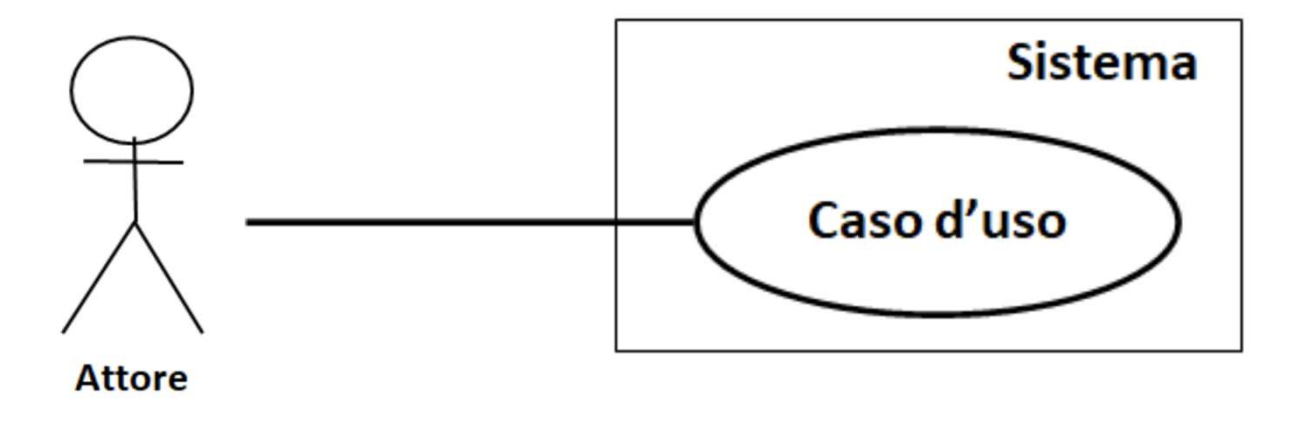
\includegraphics[scale=0.5]{img/caso.png}
\end{figure}

\subsection{Narrativa dei Casi d'Uso}
Per poter descrivere il \emph{modello dinamico}, viene redatto un documento che permette di
rappresentare gli scenari di ogni caso d'uso dal punto di vista di ogni attore coinvolto.

La descrizione di un caso d'uso segue questa struttura:

\begin{center}
    \begin{tabular}{||c||}
        \hline
        \emph{Nome} \\
        \hline
        \emph{Breve descrizione} \\
        \hline
        \emph{Attore primario} \\
        \hline
        \emph{Attori secondari} \\
        \hline
        \emph{Precondizioni} \\
        \hline
        \emph{Sequenza degli eventi principale} \\
        \hline
        \emph{Postcondizioni} \\
        \hline
        \emph{Sequenze alternative degli eventi} \\
        \hline
    \end{tabular}
\end{center}

\begin{definition}[Precondizioni e postcondizioni]
    Le \textbf{\textcolor{cyan}{precondizioni}} e le \textbf{\textcolor{cyan}{postcondizioni}} sono
    dei predicati che devono sempre essere veri in uno stato: per le \emph{precondizioni} prima di iniziare il caso d'uso,
    per le \emph{postcondizioni} alla fine. La relazione tra \emph{precondizioni}, \emph{postcondizioni} e
    sequenza principale ed alternativa ha a che fare con la \emph{logica di Hoare} \footnote{\url{https://it.wikipedia.org/wiki/Logica_di_Hoare}},
    infatti è possibile costruire la seguente \emph{tripla di Hoare}:
    \[
        \{Precondizione\} \; Sequenza \; Principale \; \{Postcondizione\}
    \]
    Ciò significa che per ogni stato $\sigma$ che soddisfa la \emph{precondizione}, se l'esecuzione della
    \emph{sequenza principale} nello stato $\sigma$ termina producendo uno stato $\sigma'$, allora la \emph{postcondizione}
    nello stato $\sigma'$ deve essere vera.

    Questo però significa che se l'esecuzione della \emph{sequenza principale} non termina o termina in modo inaspettato come indicato
    nella \emph{sequenza alternativa}, allora la \emph{postcondizione} non è garantita.
\end{definition}

\begin{definition}[Scenario]
    Uno \textbf{\textcolor{cyan}{scenario}} è un'istanza di un caso d'uso, ovvero una sequenza 
    di interazioni tra il sistema e gli attori che produce un risultato osservabile.

    Gli scenari descritti dalla \emph{sequenza degli eventi principale} sono quelli che portano
    alle \emph{postcondizioni}.
\end{definition}

La \emph{\textcolor{cyan}{sequenza degli eventi principale}} elenca i passi che compongono il caso d'uso ed ogni passo presenta la
seguente sintassi:
\begin{center}
    \verb|<numero>. <soggetto><azione><complementi>|
\end{center}
Il primo passo, inoltre, è sempre compiuto dall'\emph{attore principale}.
All'interno della sequenza possono anche presenti \emph{condizioni} e \emph{cicli}, scritti in pseudocodice.

\subsubsection{Inclusione}

L'\emph{\textcolor{cyan}{inclusione}} permette di creare una relazione di dipendenza tra casi d'uso.

Il caso d'uso \emph{incluso} può essere \emph{\textcolor{cyan}{istanziabile}} (o \emph{\textcolor{cyan}{completo}}),
quando è avviato da un attore, oppure \emph{\textcolor{cyan}{non istanziabile}}, quando viene eseguito solo quando è incluso.

\begin{figure}[h]
    \centering
    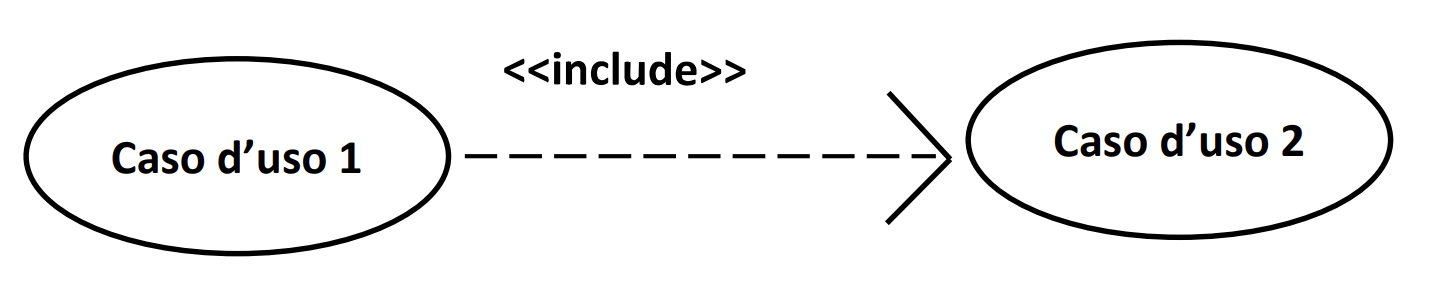
\includegraphics[scale=0.4]{img/include.png}
    \caption{Il \emph{Caso d'uso 1} include il \emph{Caso d'uso 2}.}
\end{figure}

\paragraph{Nota Bene} È importante non usare la relazione di inclusione per fare decomposizione di un caso d'uso.

\subsubsection{Estensione}

L'\emph{\textcolor{cyan}{estensione}}, a differenza dell'\emph{inclusione}, non è una dipendenza, ma
permette a un caso d'uso di incorporarne opzionalmente un altro.

\begin{figure}[h]
    \centering
    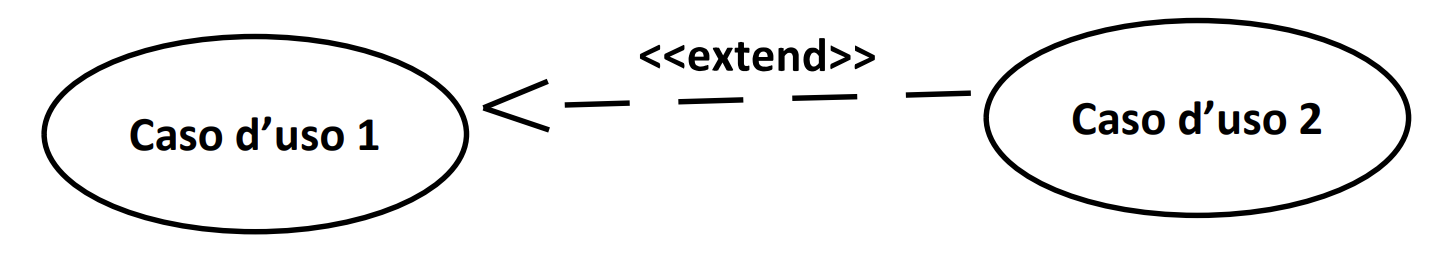
\includegraphics[scale=0.4]{img/extend.png}
    \caption{Il \emph{Caso d'uso 1} può essere esteso dal \emph{Caso d'uso 2}.}
\end{figure}

\paragraph{\textcolor{cyan}{Extension Points}}
Gli \emph{extension points} sono una notazione che permette di identificare quando
e dove inserire l'estensione. Si collega un vincolo alla freccia \verb|<<extend>>| indicando
la condizione che deve essere vera affichè l'estensione venga applicata.

\begin{figure}[h]
    \centering
    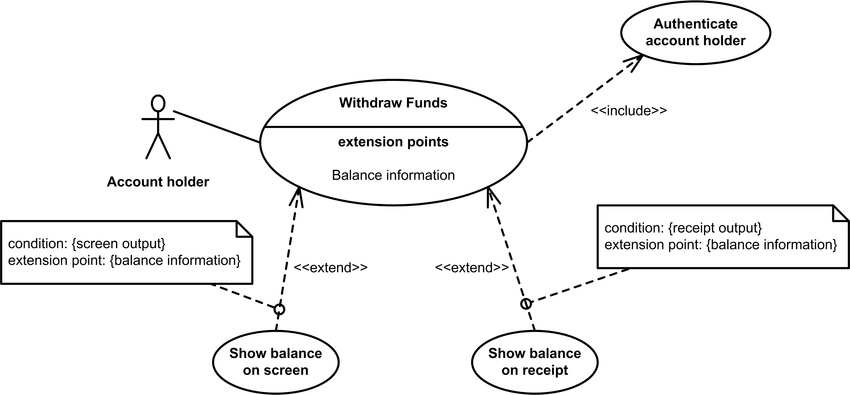
\includegraphics[scale=0.4]{img/extensionpoint.png}
\end{figure}